\section{Reconstruction from under-sampled Measurements}\label{intro}
In Signal Processing, continuous signals are represented with discrete samples. A digital recording of music, an image of a tree, or the measured velocity of a particle, all are discrete samples of continuous signals. The Nyquist-Shannon sampling rate tells us how many samples are needed to fully represent a signal: A signal which contains at most frequency $f$ should be sampled with a frequency higher than $2f$. For example if we record a piece of music where the highest tone is at 20kHz, sampling rate should be more than 40kHz. Then, the music piece gets recorded above the Nyquist-Shannon sampling rate. It is fully sampled and there is exactly one continuous signal(with maximum frequency $f$) which fits the measurement.

The Nyquist-Shannon sampling rate is not always achievable: Samples may be expensive to acquire, corrupted by noise, or incomplete by the nature of the measurement instrument. In this case we are dealing with under-sampled measurements. Many possible signals fit the measurement and from the measurement alone, we cannot distinguish the true signal from all possibilities.

With the Theory of Compressed Sensing\cite{candes2006robust}\cite{donoho2006compressed} however, we can use prior information about the signal and find the most likely candidate from all possibilities. Under the right conditions, the most likely candidate is guaranteed to be the true signal. With the Theory of Compressed Sensing, we exploit prior information to reconstruct the true signal from under-sampled measurements.

In this project, the Theory of Compressed Sensing was applied to an image reconstruction problem of Radio Astronomy. Interferometers produce under-sampled measurements of the sky which have to be reconstructed by an algorithm. A Compressed Sensing approach was developed and implemented in the Common Astronomy Software Application (CASA). The reconstruction quality was compared to standard reconstruction algorithm in astronomy on VLA data of Supernova Remnant G55.


\subsection{Image Reconstruction for Radio Interferometers}
Radio Interferometers use several antennas spaced apart from each other. Each antenna pair measures the different arrival time of a radio wave. For small field of view imaging, each antenna pair measures approximately two dimensional Fourier components of the sky (called Visibility in Astronomy). An interferometer with 26 antennas measures 325 Visibilities. The distance between the antenna pair(called a baseline) dictates which Visibility of the image gets observed. The longer the baseline, the higher frequency of the observed Visibility. The longest baseline of an interferometer is therefore a rough estimate of its maximum resolution.

For wide field of view imaging, the two dimensional Fourier relation breaks apart as additional effects dominate the measurement. This project used small field of view imaging, and the two dimensional Fourier component is a good approximation. In this document, a measured Visibilitiy equals a two dimensional Fourier component.

The interferometer only samples as many Visibilities as it has antenna pairs. The task is to reconstruct the observed image from an under-sampled Fourier space. In Astronomy, the CLEAN class of algorithms\cite{hogbom1974aperture}\cite{schwab1984relaxing}\cite{rich2008multi}\cite{rau2011multi} were developed for this task. New interferometers like MeerKAT also observe new phenomenons which, in an ideal world, can be included in the CLEAN prior and improve its reconstruction. This is not possible in CLEAN, the prior is a fixed part of the algorithm. It cannot be modified as our prior knowledge of radio images increases.

Compressed Sensing can be thought of as a generalization of the CLEAN algorithm. The prior can be exchanged without changing the rest of the reconstruction algorithm. Furthermore Compressed Sensing reconstructions may be able to find structures smaller than the antenna beam-pattern\cite{girard2015sparse}.

Antenna beam pattern. Possible super resolution: Structures smaller than the beam size of the antennas.


\subsection{Deconvolution of the Dirty Image}
The ideal interferometer would fully sample the Fourier Space and introduce no instrumental effects and the observed image can be calculated with the inverse Fourier Transform. A real world interferometer corrupts the observed image with the image with under-sampling, the antenna beam-pattern and other instrumental effects. The inverse Fourier Transform of the Visibilities can still be calculated, but it results in a corrupted "dirty" image. The observed image is convolved with a Point Spread Function (PSF) image with a Point Spread Function(PSF). The task is to reconstruct the observed image from the dirty image and the PSF, or more formally we try to solve for $x$ in equation \eqref{intro:eq:deconvolve}, where only the $PSF$ and $I_{dirty}$ are known($\star$ is used as the convolution operation).

\begin{equation}\label{intro:eq:deconvolve}
x \star  PSF + N = I_{dirty} 
\end{equation}

A deconvolution algorithm should find the observed image $x$. However, there may be many possible solutions to the equation \eqref{intro:eq:deconvolve}. Noise $N$ further complicates the deconvolution. The algorithm has to decide what is the most likely $x$ given $PSF$ and $I_{dirty}$. The PSF is specific to the interferometer. It models the sampling pattern in Fourier space, the antenna beam-pattern and more. A deconvolution algorithm is not limited to a single interferometer and can easily be used on other instruments\footnote{This is true for small field of view imaging. Wide field of view introduces additional effects that typically do not get modelled with a PSF}.

CASA produces a the dirty image and the PSF for the VLA instrument.

Note that the Formulation as a deconvolution is a valid way to solve the reconstruction problem, but it is not the only one. It was used since CASA interface is built for deconvolution algorithms. For example, it can be formulated as an in-painting problem, where only the measured Visibilities are known and the task is to find the missing Visibilities. In \ref{cs:objective} we discuss the possibilities in more details.


\begin{figure}[h!]
	\centering
	\begin{subfigure}[b]{0.28\linewidth}
		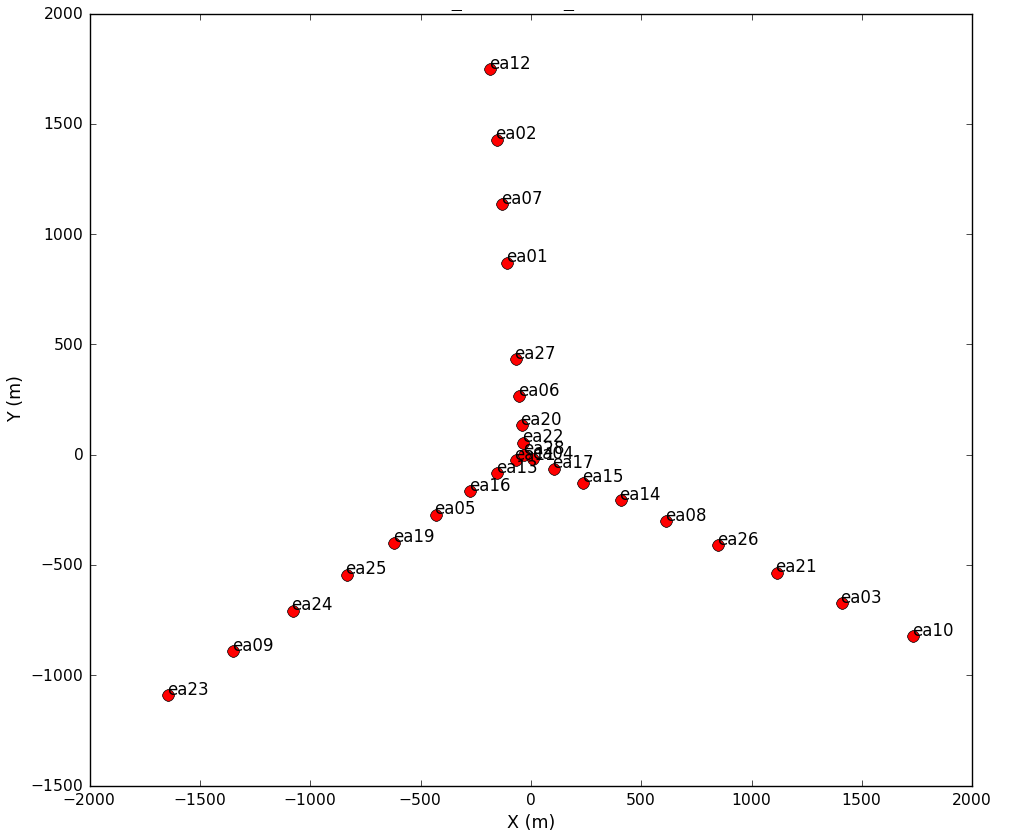
\includegraphics[width=\linewidth, trim={18px 19px 18px 18px}, clip]{./chapters/01.intro/img/antennas.png}
		\caption{Antenna Configuration}
	\end{subfigure}
	\begin{subfigure}[b]{0.28\linewidth}
		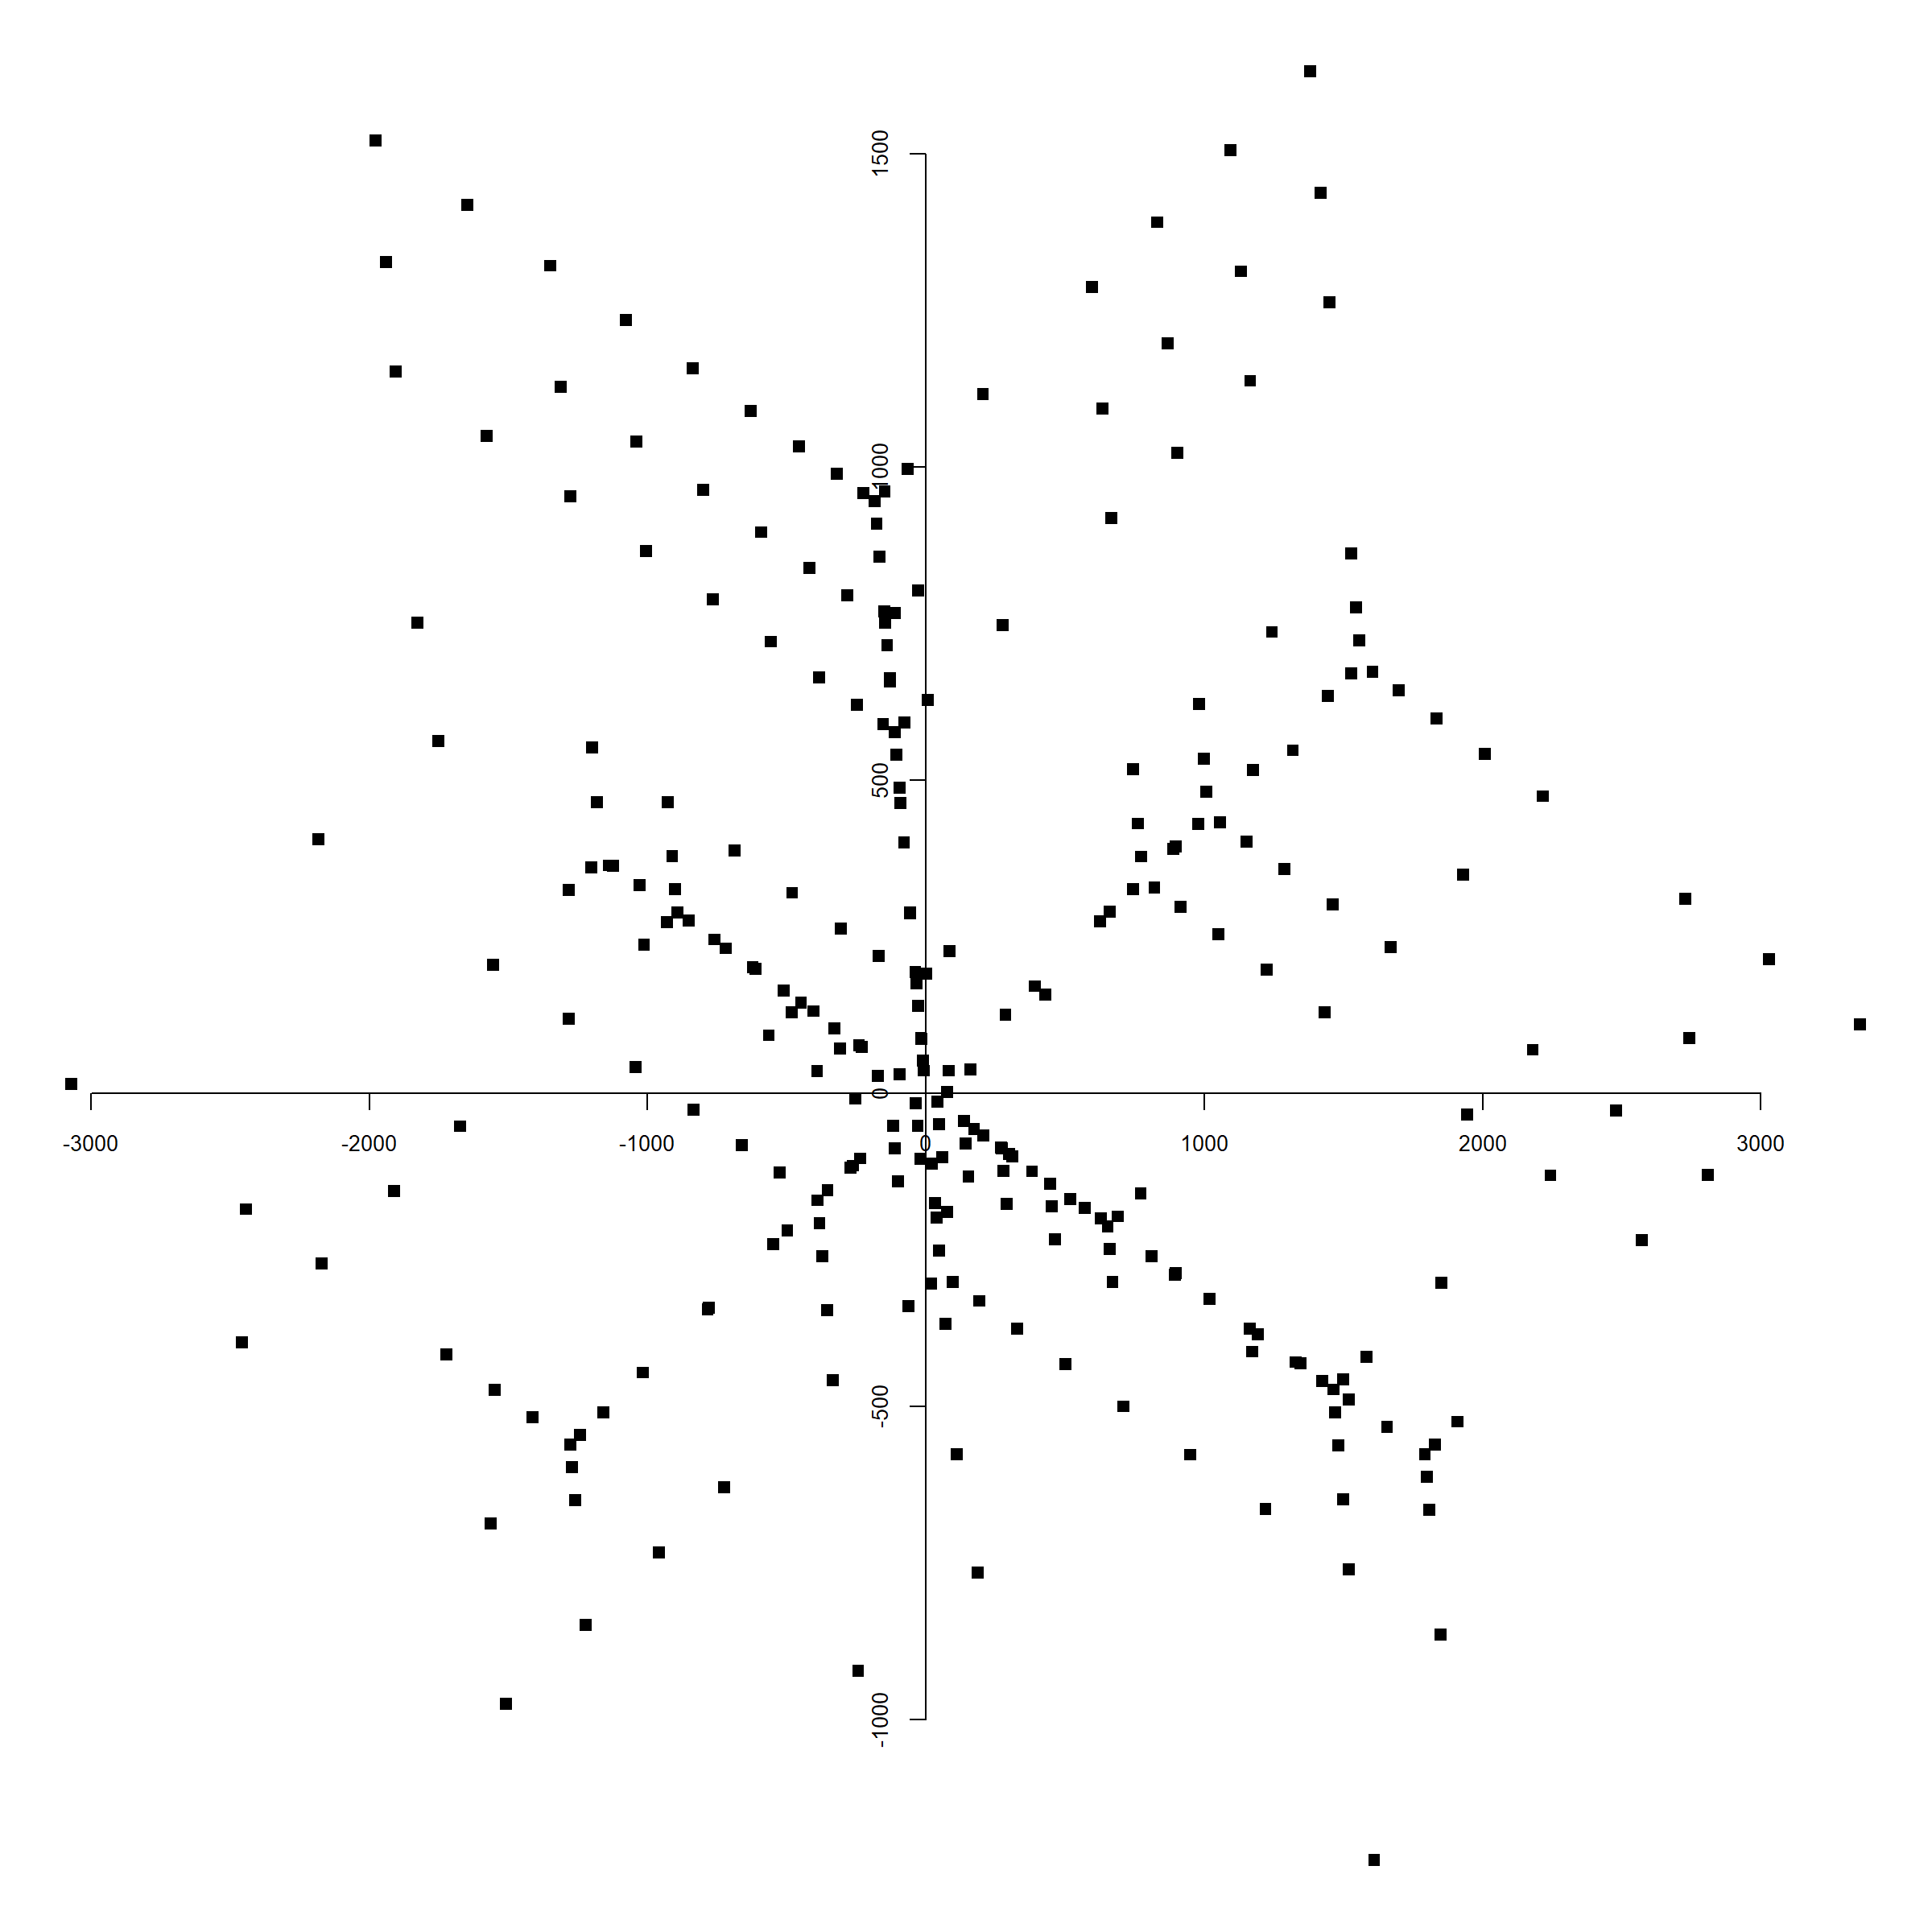
\includegraphics[width=\linewidth, trim={18px 19px 18px 18px}, clip]{./chapters/01.intro/img/uv.png}
		\caption{UV-Space}
	\end{subfigure}

	\begin{subfigure}[b]{0.28\linewidth}
		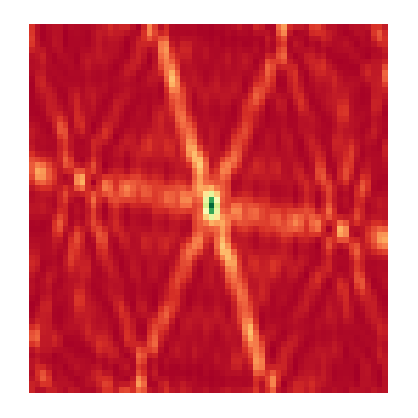
\includegraphics[width=\linewidth, trim={18px 19px 18px 18px}, clip]{./chapters/01.intro/img/psf.png}
		\caption{PSF}
	\end{subfigure}
	\begin{subfigure}[b]{0.28\linewidth}
		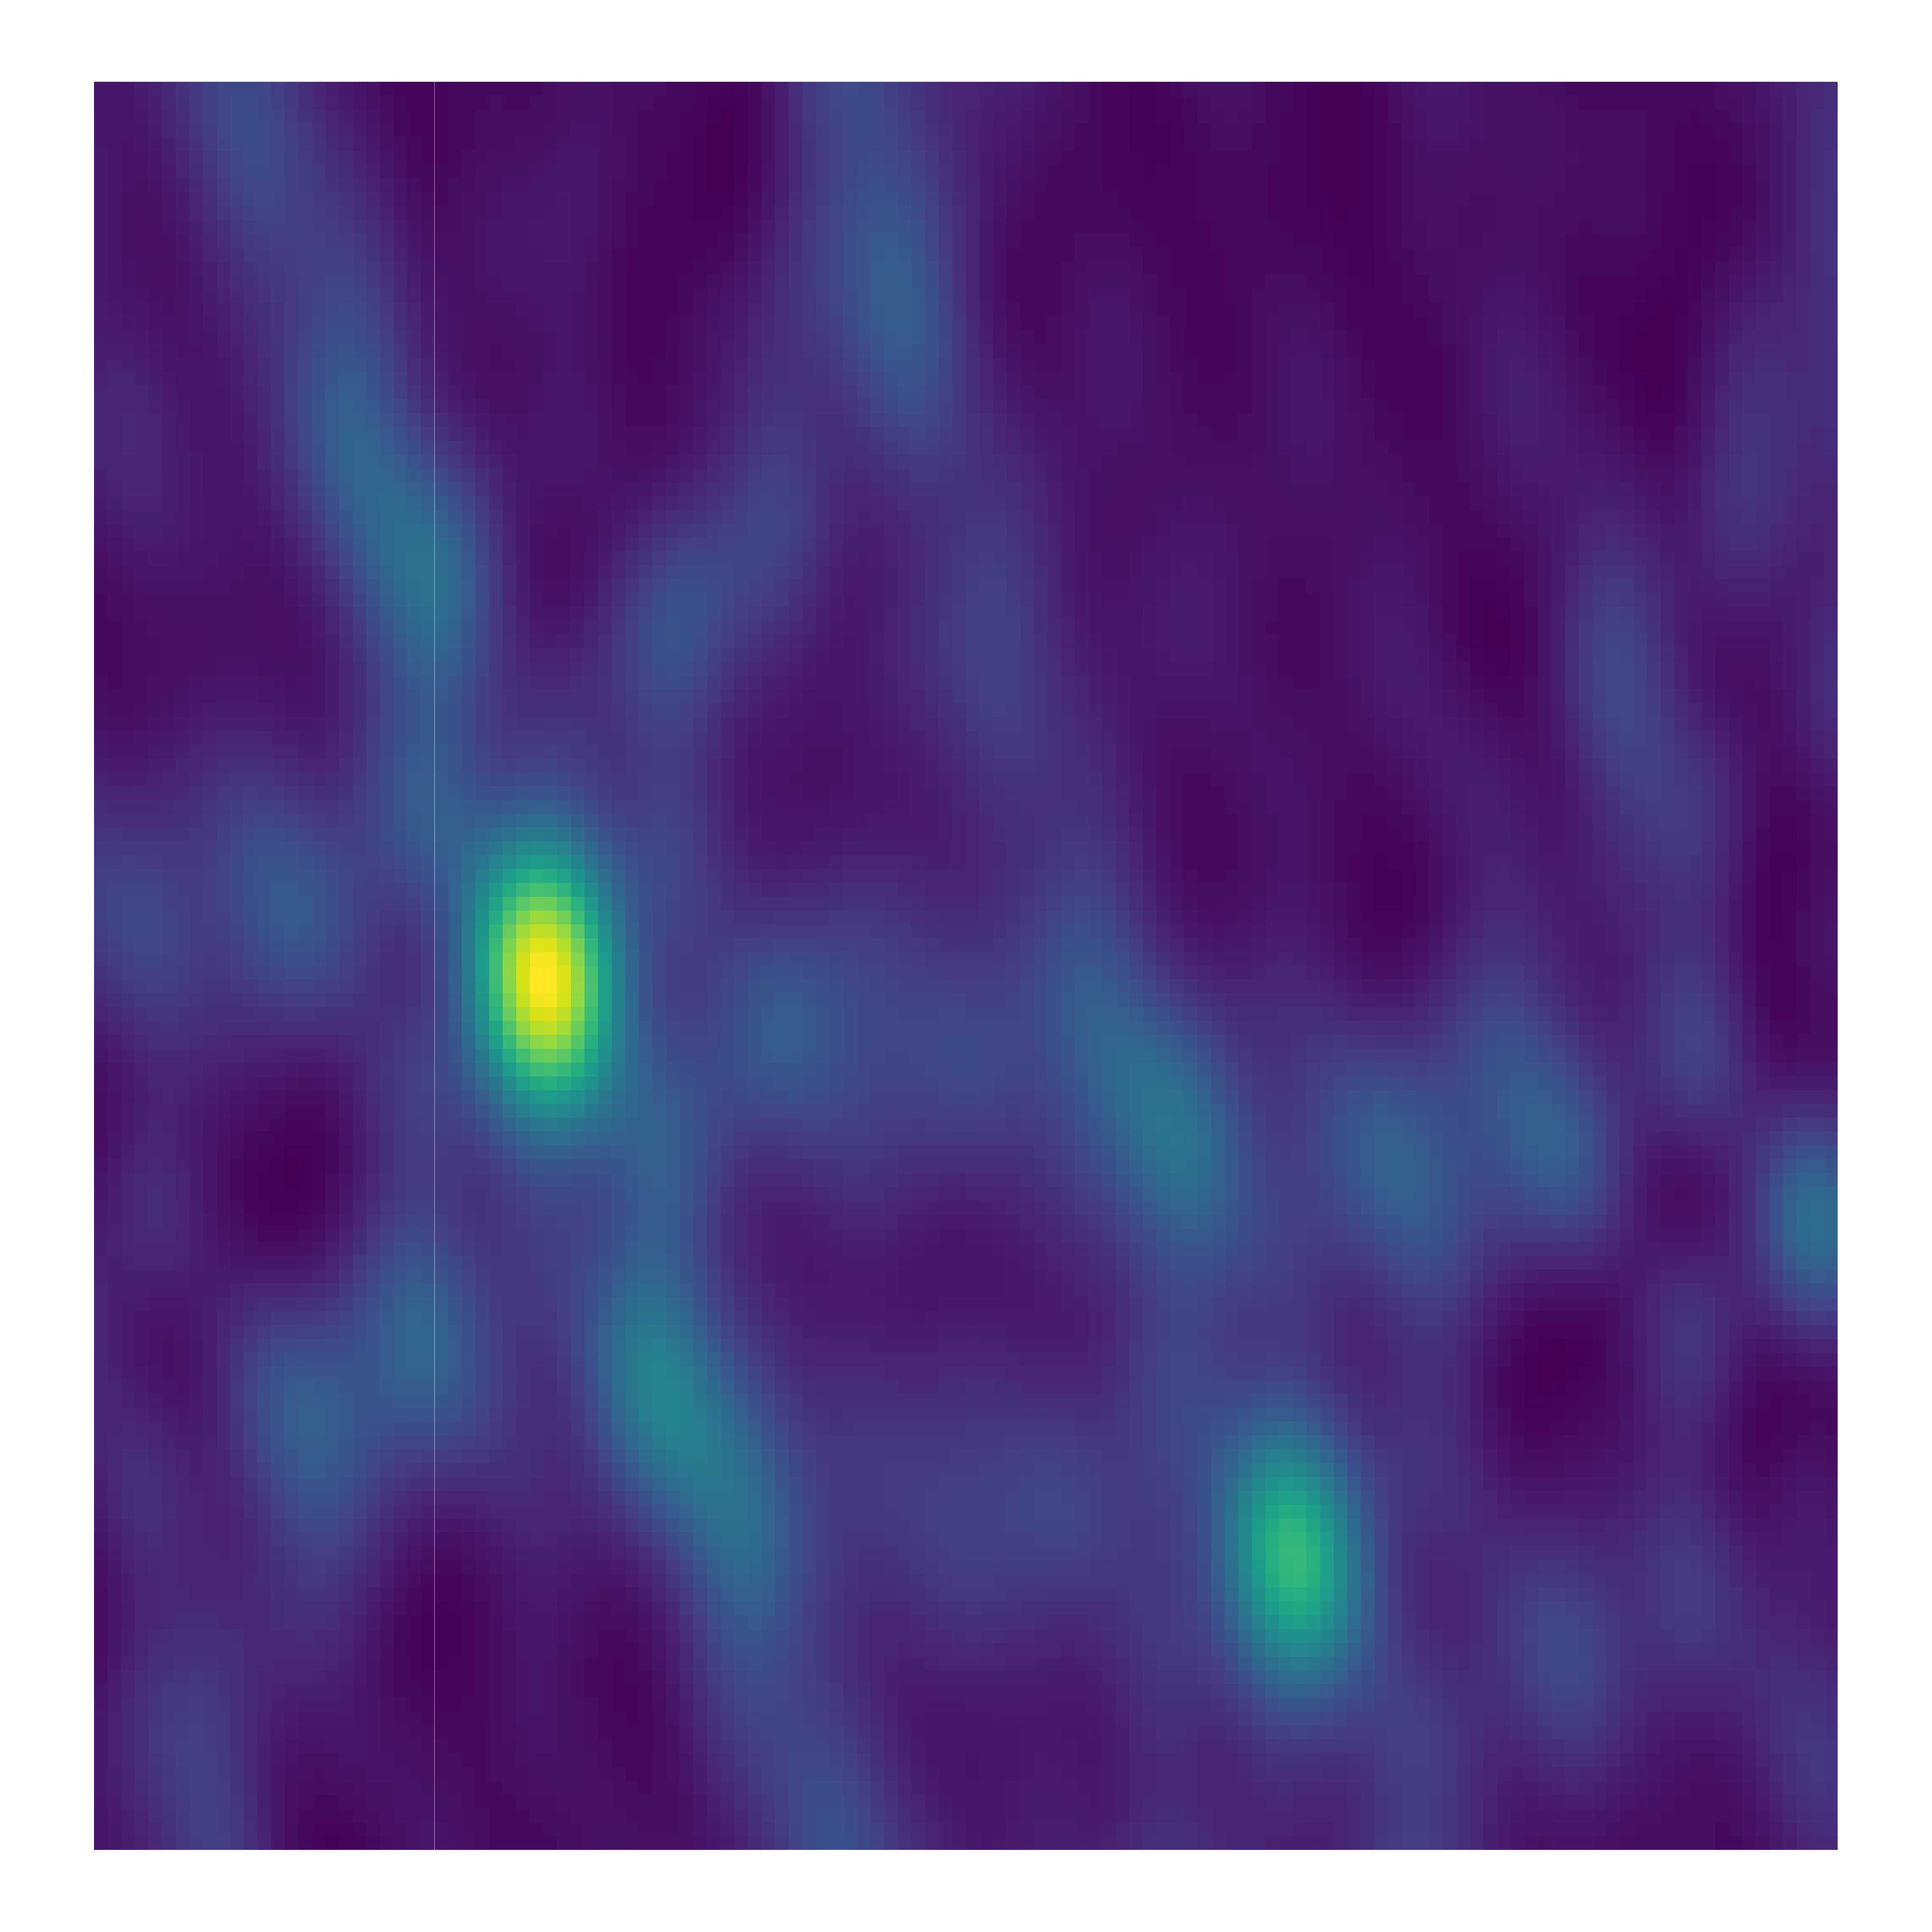
\includegraphics[width=\linewidth, trim={18px 19px 18px 18px}, clip]{./chapters/01.intro/img/dirty_image.png}
		\caption{dirty image}
	\end{subfigure}
	\begin{subfigure}[b]{0.28\linewidth}
		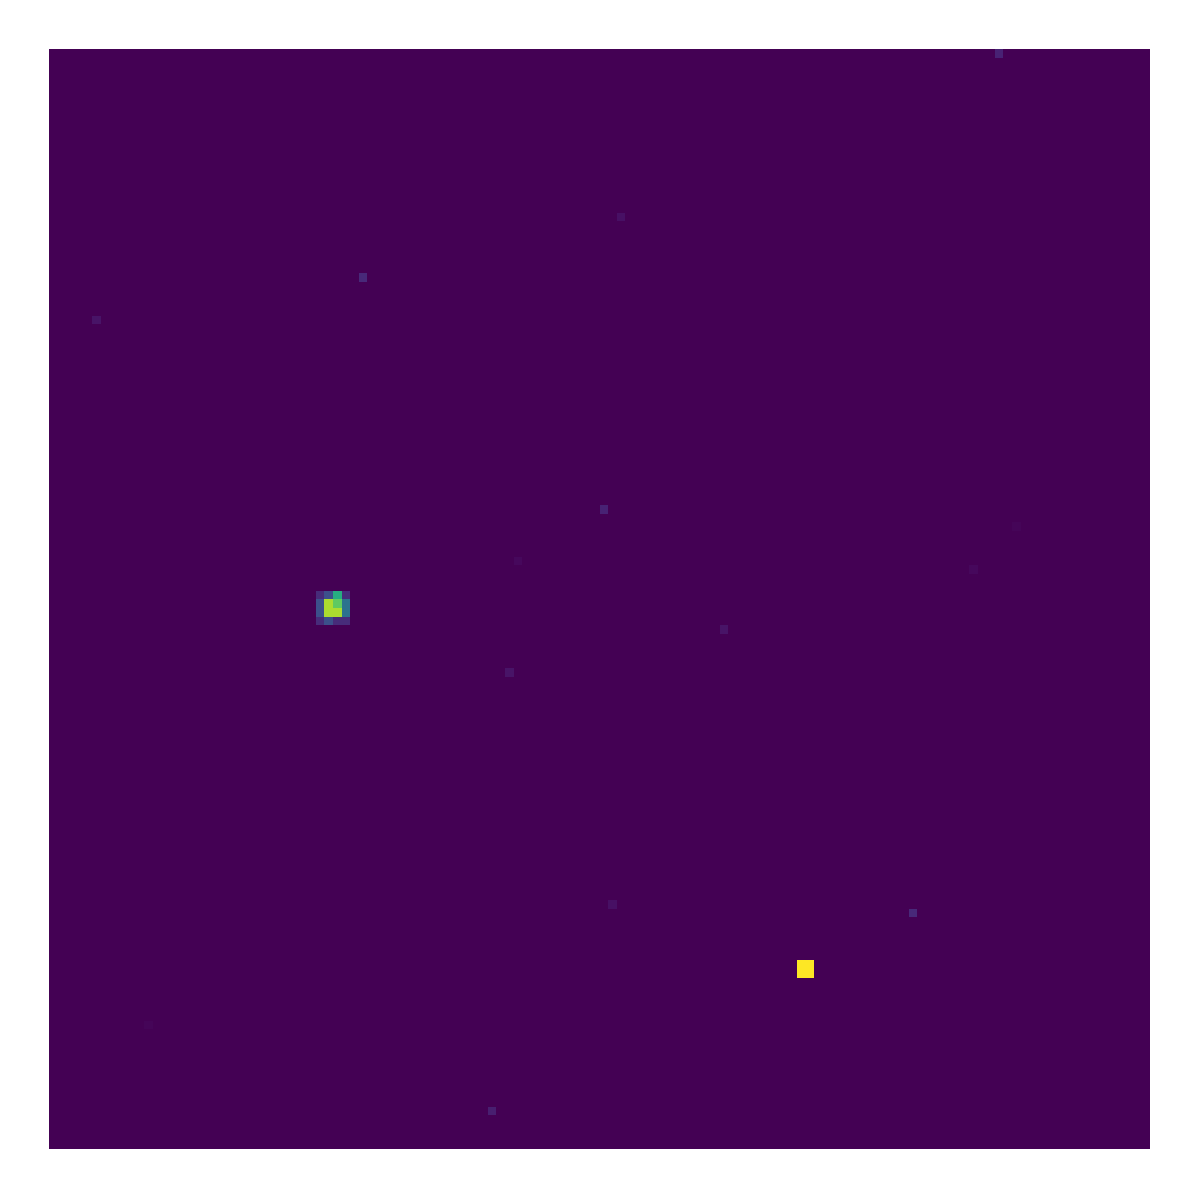
\includegraphics[width=\linewidth, trim={18px 19px 18px 18px}, clip]{./chapters/01.intro/img/true_image.png}
		\caption{true image}
	\end{subfigure}
	\caption{Deconvolution Problem VLA: Retrieve the true image when only PSF and dirty image are known}
	\label{intro:measurement_problem}
\end{figure}

\subsection{Approximation with CLEAN}
The prior of CLEAN

Fixed in the algorithm
%CLEAN assumes the observed image contains several bright point sources. 

In each iteration of CLEAN, it searches the highest peak of the dirty image and removes a fraction of the PSF. It stops until the next highest peak is below a threshold, or if the maximum number of iterations was reached. The fraction of the PSF, threshold and number of iterations are all tunable by the user.

It works as an approximation of the original problem. It greedily minimizes the objective \eqref{intro:eq:clean}. 
Note that the L0 "norm"\footnote{The L0 "norm" in this context is technically not a norm, hence the quotation marks. The L0 "norm" is a common notation in Compressed Sensing literature, therefore it is used here.} sum of non-zero elements in the image.

\begin{equation}\label{intro:eq:clean}
\underset{x}{minimize} \: \left \| I_{dirty} - x \star PSF \right \|_2^2 + \: \left \| x \right \|_0
\end{equation}

Regularization term, minimum, non-convex function (It may have local minima). 
The L0 "norm" makes this problem for non-convex: It may  it is in NP-Hard. There exist optimizer like Matching Pursuit that approximate the solution well enough for practice.

but CLEAN does not minimize to an optima, it stops early. Hard to analyse how close the current solution is to the true minimum.

Convolution with antenna beam-pattern.

CLEAN does a greedy approximation of the deconvolution problem, and assumes the resulting image consists out of a few point sources. The question remains, how close the CLEAN approximation is to the true image? If the true image consists out of a few point sources, CLEAN produces a good approximation. Extended emissions however get approximated by a large number of faint point sources. The peak of extended emissions are generally lower than of point sources. CLEAN has more trouble distinguishing extended sources from noise. Future interferometers like MeerKAT will become more sensitive to fainter sources. The reconstruction task for new instruments may contain more faint and extended sources. Ideally, we would modify the regularization of CLEAN and explicitly model the new effects. Sadly, the regularization is a fixed part of the CLEAN algorithm.


\subsection{CLEAN as Compressed Sensing Image Reconstruction}
An image reconstruction algorithm in the Compressed Sensing Framework consists of three parts:

\begin{itemize}
	\item A prior function $p()$.
	\item An optimization algorithm.
	\item An objective with a data and regularization term.
\end{itemize}

CLEAN is a Compressed Sensing Reconstruction algorithm with specific choices for prior, optimization algorithm. and objective. The prior $p()$ in CLEAN is the L0 "norm", Matching Pursuit as the optimization algorithm. The objective from CLEAN needs a additional parameter $\lambda$.  [which represents the trade-off between deconvolution and regularization.] the more noisy it is, the more regularization is needed. We arrive at the similar \eqref{intro:eq:csclean}.

\begin{equation}\label{intro:eq:csclean}
\underset{x}{minimize} \: \left \| D_{dirty} - x \star PSF \right \|_2^2 \: + \: \lambda \: p(x) 
\end{equation}

All that was changes was an additional parameter $\lambda$, so why would one want to do this? 
Applying non-convex optimization techniques,
Theoretical guarantees of compressed Sensing.
Replacing $p()$ with anything else

Now we can minimize \eqref{intro:eq:csclean} with non-convex optimization techniques, we can analyse how calculate lower limits for the objective.


We assume $x$ assumes the $x$ contains a few point sources. In Compressed Sensing terminology, it assumes $x$ is sparse in image space. Since $x$ is already an image.


Compressed sensing reconstruction is able to reconstruct the observation even from undersampled measurements. Even though shannon-nyquist theorem is higher.

The guarantees of Compressed Sensing Reconstruction: Incoherent from the measurement space and sparse space is sparse.

Incoherence is easy. Interferometers measure in the Fourier space(This is an approximation for small field of view imaging. The approximation breaks apart in wide field of view). The image space is maximally incoherent from the Fourier space. Intuitively, A change in a single pixel will change all fourier components. A change in a single fourier component, changes all pixels.

maximize the information gained for each element in the sparse space.

The sparse space is here to distinguish true image from unlikely candidates. It models our prior knowledge.

Then, one can reconstruct the true image from undersampled measurements. How many measurements are needed? that depends on how sparse it is. 

Taking again CLEAN as an example, if we know the image contains only one point source, we can locate it with only a few Visibilities. However if the image contains many point sources located closely together, we need more Visibilities.

The average case analysis is not trivial, 

The prior and the optimization algorithm are disconnected and the prior $p()$ can be replaced for example with the L2 norm.

%In the Compressed Sensing Framework, an approach is split into three separate parts. To demonstrate the flexibility of the Compressed Sensing Framework, we convert CLEAN into a Compressed Sensing approach.

% First we add a regularization term to \eqref{intro:eq:clean} and arrive at the new objective \eqref{intro:eq:csclean}. The objective contains the original CLEAN data term and a new regularization term. The data term forces the reconstruction to be close to the measurement, while the regularization term forces the reconstruction to be plausible. $\lambda$ models the expected noise in the problem. Note that the $\left \| Px \right \|_0$ acts as an indicator function. 

%The last step is choosing a similar optimization algorithm: In every iteration, CLEAN searches the highest peak in the dirty image. Matching Pursuit is a greedy optimization algorithm. In every iteration it searches the step which minimizes \eqref{intro:eq:csclean} the most. This Compressed Sensing approach is similar to CLEAN, but the new objective has a unique global minimum even with the presence of noise. The tunable parameters of CLEAN are replaced by a single parameter $\lambda$. 

%The strength of Compressed Sensing Framework is its flexibility: The CLEAN prior works well on point sources, but is not ideal for extended emissions. In this Framework, the prior $P$ can be replaced without changing the objective or the optimization algorithm. This has led to increased interest in Compressed Sensing for wide Field of View imaging.




